\documentclass{beamer}
%
% Choose how your presentation looks.
%
% For more themes, color themes and font themes, see:
% http://deic.uab.es/~iblanes/beamer_gallery/index_by_theme.html
%
\mode<presentation>
{
  \usetheme{default}      % or try Darmstadt, Madrid, Warsaw, ...
  \usecolortheme{default} % or try albatross, beaver, crane, ...
  \usefonttheme{default}  % or try serif, structurebold, ...
  \setbeamertemplate{navigation symbols}{}
  \setbeamertemplate{caption}[numbered]
  %\setbeamertemplate{footline}[frame number]
}
\usepackage{outlines}
 
\usepackage{graphicx}
\usepackage[english]{babel}
\usepackage[utf8x]{inputenc}
\title{Modeling Module 1}
\setbeamertemplate{footline}[frame number]
%\author{Instructor; M.K. Srivas \\
%TA: Zubin Duggal}

\begin{document}
\begin{frame}
  \titlepage
\end{frame}

% Uncomment these lines for an automatically generated outline.
%\begin{frame}{Outline}
%  \tableofcontents
%\end{frame}

\section{Outline}


\begin{frame}{}
\begin{itemize}
\item 
\end{itemize}

\end{frame}

\begin{frame}{}
%\uncover<1->{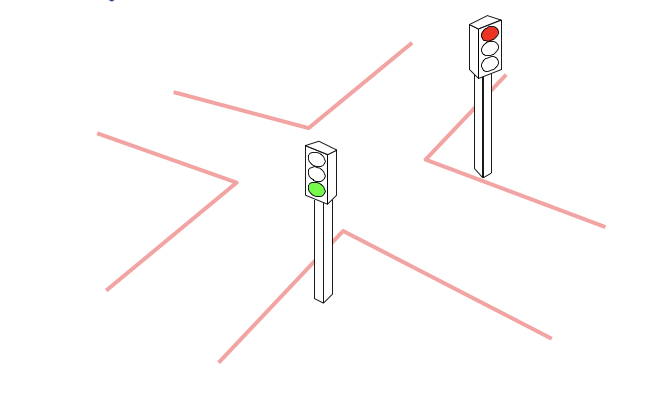
\includegraphics[scale=0.3]{pics/trafficsignal.png}}\hfill
\end{frame}

\begin{frame}{}

\end{frame}

\begin{frame}{}

\end{frame}

\begin{frame}{Some Definitions}
\begin{itemize}
\uncover<1->{\item Bounded Satisfaction of a path: $\pi {\models}_k \phi$ }\\
\begin{itemize}
\uncover<1->{\item SAT of $\pi$ requires inspecting only a $k$-long (or shorter) $\pi$-prefix \\
\item $\pi$ is $k$-bounded lasso $\implies$ $\pi {\models}_k \phi$}
\end{itemize}

\uncover<2->{\item Bounded satisfaction by a TS $M$: $M \models_k \phi $} \\
\begin{itemize}
\uncover<2->{\item every lasso-shaped  $k$-bounded path $\pi$ in $M$ satisfies $\phi$}
\end{itemize}

\uncover<3->{\item A $Completeness Threshold ~(CT)~K$ for an $(M, \phi)$ is a $K$ s.t.: }
\begin{itemize}
\uncover<3->{\item $M \models_K \phi \implies M\models \phi$}
    \uncover<4->{\item why should such a $K$ exist at all?}
\end{itemize}

\end{itemize}
\end{frame}


\end{document}
